% Plantilla FCFM/UChile (clase umemoria, dccuchile/memoria-tesis-latex).
% Para compilar en Overleaf: subir esta carpeta y usar pdfLaTeX como compilador.
% Para una memoria en ingles: agregar la opcion [english] y borrar el .aux.
\documentclass{umemoria}

\depto{Departamento de Ciencias de la Computación}
\author{Agustín Sebastián Solís Meza}
\title{Bases y análisis de discrepancias entre el discurso de los partidos políticos y la práctica de sus representantes parlamentarios}

% Memoria de pregrado (Ingeniero/a Civil en Computación).
\memoria{Ingeniero Civil en Computación}
% \tesis{Magíster en ???} % incluir solo en caso de doble titulación

% En una memoria solo puede haber un profesor guía.
\guia{Valentin Barriere}

% En una memoria el co-guía aparece como primer integrante de la comisión.
% \coguia{Franziska Wagner} % este comando es solo para co-guía de *tesis*

% Integrantes de la comisión (el primero es la co-guía Franziska Wagner).
% Completar con nombres y apellidos completos de los demás integrantes.
\comision{Franziska Wagner,Nombre Completo Integrante Dos,Nombre Completo Integrante Tres}

% \auspicio{Nombre Institución} % incluir si el trabajo recibió financiamiento (p. ej. CENIA)

% Año del examen de título (defensa). Por defecto usa el año actual.
\anho{2026}

% La clase umemoria ya carga inputenc (utf8), geometry, babel (spanish), graphicx, etc.
\usepackage{booktabs} % tablas con \toprule, \midrule, \bottomrule
\usepackage{float}    % opción [H] para fijar figuras/tablas

\begin{document}

\frontmatter
\maketitle

\begin{resumen}
% Resumen ejecutivo en una sola página: justificación, objetivos, método y hallazgos.
% TODO: redactar al final, cuando los resultados estén consolidados.
En las democracias representativas existe una brecha potencial entre lo que los
partidos políticos \emph{declaran} en sus programas y discursos y lo que sus
representantes \emph{hacen} al legislar. Este trabajo construye bases de datos
públicas y comparables sobre la actividad de los diputados de la Asamblea Nacional
francesa (XV legislatura, 2017--2022) ---programas electorales, intervenciones en
el hemiciclo, actividad en Twitter, y votaciones sobre leyes y enmiendas--- y
aplica modelos de procesamiento de lenguaje natural (clasificación supervisada
MARPOR con ManifestoBERTa y modelado de tópicos con BERTopic) para caracterizar y
contrastar la \emph{agenda declarada} (énfasis temático) con la \emph{agenda
revelada} (soporte por el voto) de cada partido. Los resultados muestran que [\dots].
\end{resumen}

% Para tesis en inglés, incluir también el abstract:
%\begin{abstract}
%\end{abstract}

\begin{dedicatoria}
% Optativo, estructura libre.
\end{dedicatoria}

\begin{thanks}
% Agradecimientos (optativo).
\end{thanks}

\tableofcontents
\listoftables  % opcional
\listoffigures % opcional

\mainmatter

\chapter{Introducción}
\label{cap:introduccion}

% La introducción responde a ¿qué? y ¿por qué?: contexto, justificación, objetivos,
% alcances, método (a grandes rasgos) y estructura de la memoria.

\section{Contexto y motivación}
\label{sec:contexto}
% En las democracias representativas los partidos comunican sus valores mediante
% programas y discursos públicos, pero a menudo hay discrepancias entre lo que
% declaran y lo que hacen sus representantes. Por qué importa: confianza, transparencia.

\section{Descripción del problema}
\label{sec:problema}
% El desfase declarado/práctica está poco medido empíricamente; las fuentes están
% dispersas y en formatos heterogéneos; los estudios suelen mirar una sola dimensión.

\section{Objetivos}
\label{sec:objetivos}

\subsection{Objetivo general}
\label{sec:objetivo-general}
% Construir y analizar bases de datos públicas que permitan detectar y describir
% discrepancias entre el discurso programático de los partidos y la práctica
% parlamentaria de sus representantes.

\subsection{Objetivos específicos}
\label{sec:objetivos-especificos}
% 1. Recolectar y organizar fuentes (redes sociales, programas, datos parlamentarios).
% 2. Construir una base de programas partidarios comparable (MPDB).
% 3. Recolectar y estructurar información parlamentaria (intervenciones, votaciones).
% 4. Estandarizar y unificar las bases en un formato apto para análisis computacional.
% 5. Aplicar modelos de NLP (clasificación MARPOR, modelado de tópicos) sobre los corpus.
% 6. Identificar y cuantificar discrepancias entre lo declarado y lo revelado por el voto.

\section{Alcances}
\label{sec:alcances}
% Qué cubre y qué no: foco en Francia (XV legislatura 2017-2022); 5 corpus;
% análisis a nivel de partido; limitaciones de cobertura y de los datos.

\section{Estructura de la memoria}
\label{sec:estructura}
% Breve mapa de los capítulos siguientes.

\chapter{Marco teórico y revisión de la literatura}
\label{cap:marco-teorico}

% Responde a ¿cómo? y ¿con qué herramientas?: define los conceptos clave del trabajo.

Este capítulo define los conceptos y las herramientas sobre los que se apoya el
resto de la memoria, siguiendo una lógica deductiva que va de las nociones
generales a los instrumentos concretos. Primero se precisan las ideas de agenda
temática, \emph{salience} y coherencia partidaria, y la distinción entre lo que
un partido declara y lo que revela al votar, que es la pregunta que articula el
trabajo. Luego se presenta la taxonomía del \emph{Manifesto Project} (MARPOR)
como espacio de categorías políticas comparable entre fuentes, junto con el índice
posicional RILE y las encuestas de expertos que sirven de referencia externa.
Por último se revisan las técnicas de procesamiento de lenguaje natural que
permiten clasificar texto político a gran escala. Estos conceptos preparan la
metodología del capítulo~\ref{cap:metodologia} y la lectura de los hallazgos del
capítulo~\ref{cap:resultados}, pero aquí no se presentan resultados del caso
estudiado.

\section{Discurso político, agenda y coherencia partidaria}
\label{sec:discurso-coherencia}

El estudio del comportamiento partidario distingue de manera habitual entre lo
que un partido \emph{dice} y lo que un partido \emph{hace}. La primera dimensión
remite a la \textbf{agenda declarada}, es decir, al conjunto de temas que una
organización política decide poner en primer plano en su comunicación pública, ya
sea en su programa electoral, en los medios o en el debate parlamentario. La
segunda remite a la \textbf{agenda revelada}, esto es, a las posiciones que el
partido expresa cuando sus representantes votan sobre textos concretos. Ambas son
observables, pero no son equivalentes, y su contraste es el problema central de
esta memoria.

Un concepto útil para caracterizar la agenda declarada es el de \emph{salience},
la prominencia relativa que un actor otorga a cada tema. La literatura sobre
competencia partidaria sostiene que los partidos compiten menos tomando
posiciones opuestas sobre los mismos asuntos y más enfatizando selectivamente
aquellos temas en los que se sienten fuertes, una idea vinculada a la noción de
\emph{issue ownership}, la asociación duradera entre un partido y ciertos temas.
Desde esta perspectiva, describir una agenda es, ante todo, medir de qué se habla
y cuánto, antes que ubicar al actor en una escala de posiciones.

Esta óptica temática tiene una consecuencia metodológica importante. Reducir a un
partido a un único punto en un eje izquierda--derecha resume su posición, pero
pierde la estructura de su agenda y resulta frágil cuando el objeto de interés es
la coherencia entre discurso y voto. La ciencia política comparada ha mostrado,
además, que la competencia europea no se ordena solo por el eje económico, sino
también por una segunda dimensión que opone valores libertarios, alternativos y
cosmopolitas a posiciones tradicionales, autoritarias y nacionalistas, conocida
como dimensión GAL--TAN \cite{hooghe2002galtan}. Un enfoque basado en el énfasis
por temas permite captar esa multidimensionalidad, que un índice unidimensional
tiende a aplanar.

La agenda declarada, sin embargo, no se expresa igual en todas partes. Un mismo
partido se dirige a audiencias distintas en su programa, en las redes sociales y
en el hemiciclo, y adapta a cada canal tanto el registro como la selección de
temas, de modo que el canal opera como un condicionante estructural de lo que se
observa \cite{ivanusch2024channels}. Comparar la agenda de un partido consigo
misma a través de canales, y no solo entre partidos, se vuelve entonces una
pregunta con contenido propio.

Del lado de la agenda revelada, el estudio del voto legislativo aporta un segundo
cuerpo de conceptos. En los sistemas parlamentarios, el voto rara vez es la suma
de decisiones individuales independientes: los grupos exhiben una fuerte
\textbf{disciplina de bloque}, sostenida por incentivos organizativos y por la
lógica de gobierno frente a oposición \cite{sieberer2006partyunity}. La unidad de
voto observada es, en consecuencia, el resultado de principales en competencia,
como el partido, el electorado y el gobierno, más que un reflejo directo de las
preferencias temáticas de cada representante \cite{carey2007competing}. Esta
distinción anticipa una idea que la memoria retoma más adelante: el voto puede
revelar sobre todo una posición de bloque y, solo en ciertos márgenes, una señal
temática propia. El contraste sistemático entre la agenda declarada y la revelada,
sobre un mismo conjunto de actores y bajo una taxonomía común, es precisamente el
vacío que este trabajo busca ocupar.

\section{El Manifesto Project y la taxonomía MARPOR}
\label{sec:marpor}

Para comparar el contenido político de fuentes tan distintas como un programa
electoral, un mensaje en redes o un texto legislativo se necesita un espacio de
categorías común. Esta memoria adopta el esquema del \emph{Manifesto Project}
(MARPOR) \cite{marpor_mp_v5}, un estándar consolidado de la ciencia política
comparada con el que se han codificado manualmente programas electorales de
numerosos países durante décadas. Su unidad de análisis es la \emph{cuasi-frase},
un fragmento que expresa una única idea política, a la que se asigna una
categoría temática.

El esquema organiza el contenido en \textbf{56 categorías} agrupadas en
\textbf{siete dominios} macro. El dominio se obtiene del primer dígito del código
de categoría, lo que habilita una lectura jerárquica: fina a nivel de categoría y
más robusta a nivel de dominio. El Cuadro~\ref{tab:marpor-dominios} resume los
siete dominios con una categoría de ejemplo cada uno; el listado completo de las
56 categorías se recoge en el anexo~\ref{anexo:marpor}.

\begin{table}[H]
\centering
\caption{Los siete dominios de la taxonomía MARPOR, con una categoría ilustrativa
por dominio. El detalle de las 56 categorías se encuentra en el
anexo~\ref{anexo:marpor}.}
\label{tab:marpor-dominios}
\small
\begin{tabularx}{\textwidth}{@{}l l >{\raggedright\arraybackslash}X@{}}
\toprule
\textbf{Dominio} & \textbf{Nombre (MARPOR)} & \textbf{Categoría de ejemplo} \\
\midrule
1 & External Relations & Internacionalismo \\
2 & Freedom and Democracy & Libertad y derechos humanos \\
3 & Political System & Autoridad política \\
4 & Economy & Economía de libre mercado \\
5 & Welfare and Quality of Life & Expansión del Estado de bienestar \\
6 & Fabric of Society & Ley y orden \\
7 & Social Groups & Grupos laborales \\
\bottomrule
\end{tabularx}
\end{table}

Tres propiedades hacen de MARPOR un espacio idóneo para este trabajo. Es
\emph{independiente de la fuente}, porque las mismas categorías se aplican por
igual a distintos tipos de texto; es \emph{citable y externamente validable}, al
ser un estándar internacional cuyas estimaciones pueden contrastarse contra
codificaciones humanas y encuestas de expertos; y admite una \emph{lectura tanto
temática como posicional}, pues las distribuciones de categorías sostienen el
análisis de énfasis y, al mismo tiempo, permiten derivar un índice de posición
cuando se lo necesita.

Ese índice es el \textbf{RILE} (\emph{right--left}), propuesto por Laver y Budge
\cite{laver1992party}, que resume la posición de un partido como la diferencia
entre el porcentaje de cuasi-frases asignadas a un conjunto canónico de
categorías de derecha y el de un conjunto de categorías de izquierda. El RILE es
un resumen conveniente, pero tiene límites conceptuales conocidos: es
\emph{unidimensional}, de modo que colapsa en un solo eje una agenda que suele ser
multidimensional, y es \emph{ciego a la dirección} del enunciado, ya que cuenta
del mismo modo el apoyo y el ataque a una misma idea. Por estas razones, en esta
memoria el RILE no es el instrumento del análisis sustantivo, sino que se reserva
para \emph{validar} el pipeline; el análisis principal se construye sobre el
\textbf{énfasis por dominio}, es decir, sobre las distribuciones temáticas
completas y no sobre un índice posicional colapsado.

La validación posicional se apoya en una referencia externa e independiente del
texto: el \emph{Chapel Hill Expert Survey} (CHES), una encuesta que sitúa a los
partidos europeos en distintas dimensiones a partir del juicio de expertos. Se
emplea la edición de 2019 \cite{jolly2022ches, ches2019data}; existe una edición
más reciente de 2024 \cite{rovny2025ches}, que no se utiliza aquí. CHES cumple en
este trabajo un papel estrictamente de \emph{benchmark} externo con el cual
contrastar las posiciones estimadas, y no el de una taxonomía que oriente el
análisis temático.

\section{Procesamiento de lenguaje natural para texto político}
\label{sec:nlp-politico}

Codificar manualmente cinco corpus con el esquema MARPOR sería inviable por su
volumen, de modo que la asignación de categorías se automatiza con técnicas de
procesamiento de lenguaje natural. Se combinan dos enfoques complementarios: una
clasificación supervisada, que asigna las categorías teóricas del esquema, y un
modelado de tópicos no supervisado, que descubre agrupaciones empíricas dentro de
cada corpus. Ambos se describen a continuación en el plano conceptual; su
configuración concreta se detalla en el capítulo~\ref{cap:metodologia}.

\subsection{Clasificación supervisada: ManifestoBERTa}
\label{sec:manifestoberta}

La clasificación supervisada parte de un modelo de lenguaje preentrenado que se
afina para una tarea específica. El núcleo del análisis emplea ManifestoBERTa
\cite{manifestoberta2024}, un modelo publicado por el propio Manifesto Project que
clasifica cuasi-frases en las 56 categorías del esquema MARPOR. Está construido
sobre XLM-RoBERTa \cite{conneau2020xlmr}, un modelo multilingüe preentrenado sobre
texto de numerosos idiomas, lo que resulta apropiado para un corpus en francés y
permite aprovechar representaciones lingüísticas transferibles entre lenguas.

Un supuesto conceptual debe hacerse explícito. ManifestoBERTa fue entrenado sobre
programas electorales, un género con un registro particular, de manera que
aplicarlo a otras superficies, como mensajes en redes, intervenciones
parlamentarias o textos legislativos, constituye una \textbf{transferencia de
dominio}. Esa transferencia es razonable, porque la taxonomía es temática y no
depende del formato, pero no es gratuita, y por eso el desempeño del clasificador
fuera de su dominio de origen debe evaluarse antes de interpretar cualquier
resultado. La forma de esa evaluación se desarrolla en la
sección~\ref{sec:metodo-manifestoberta}.

\subsection{Modelado de tópicos no supervisado: BERTopic}
\label{sec:bertopic}

Como complemento exploratorio se utiliza BERTopic \cite{grootendorst2022bertopic},
una técnica de modelado de tópicos que, en lugar de imponer categorías teóricas,
descubre agrupaciones de documentos a partir de su similitud semántica. Su lógica
encadena varias etapas: representa cada documento como un vector denso mediante
\emph{embeddings} de oraciones \cite{reimers2019sentencebert}, reduce la
dimensionalidad de esos vectores con UMAP \cite{mcinnes2018umap}, agrupa los
documentos con un algoritmo de \emph{clustering} basado en densidad, HDBSCAN
\cite{mcinnes2017hdbscan}, y describe cada grupo con sus términos más
característicos.

El papel de BERTopic en esta memoria es \textbf{exploratorio y no comparable entre
arenas}. Como los tópicos emergen de cada corpus por separado, no constituyen un
espacio común entre fuentes ni permiten contrastar partidos de manera sistemática,
a diferencia de la clasificación supervisada sobre MARPOR. Por ello se emplea para
inspeccionar qué temas afloran en el texto y para detectar ruido o lenguaje
procedimental, pero no para sostener conclusiones cuantitativas. Su configuración
se detalla en la sección~\ref{sec:metodo-bertopic}. El
Cuadro~\ref{tab:nlp-comparacion} resume la complementariedad conceptual de ambos
enfoques.

\begin{table}[H]
\centering
\caption{Comparación conceptual de los dos enfoques de clasificación de texto
empleados en el trabajo.}
\label{tab:nlp-comparacion}
\small
\begin{tabularx}{\textwidth}{@{}l >{\raggedright\arraybackslash}X >{\raggedright\arraybackslash}X@{}}
\toprule
 & \textbf{ManifestoBERTa (supervisado)} & \textbf{BERTopic (no supervisado)} \\
\midrule
Categorías & Fijas y teóricas (esquema MARPOR) & Emergentes del propio corpus \\
Comparabilidad entre arenas & Alta (espacio común) & Baja (tópicos por corpus) \\
Rol en el trabajo & Núcleo del análisis & Complemento exploratorio \\
\bottomrule
\end{tabularx}
\end{table}

\subsection{Detección de postura y marcos de valores}
\label{sec:stance-valores}

Existen enfoques que apuntan a dimensiones del texto político distintas del tema.
La \emph{detección de postura} busca determinar si un texto está a favor o en
contra de un objetivo, y se ha desarrollado, por ejemplo, sobre plataformas de
democracia participativa y consultas públicas europeas
\cite{barriere2022cofe, barriere2023multilingual}. Los \emph{marcos de valores}
ofrecen otra lente complementaria, ya sea a través de la teoría de valores básicos
de Schwartz \cite{schwartz2012overview} o de la teoría de los fundamentos morales
\cite{graham2013moral}, que caracterizan el discurso según los valores o
principios que moviliza. Estos enfoques son afines al problema de esta memoria,
pero quedan \textbf{fuera de su alcance}: el análisis se concentra en el énfasis
temático bajo la taxonomía MARPOR, y la incorporación de la postura o de los
marcos de valores se deja señalada como línea de trabajo futuro.

\section{Trabajos relacionados}
\label{sec:trabajos-relacionados}

La pregunta por la coherencia entre lo que los partidos declaran y lo que hacen
tiene una larga tradición en la ciencia política, que ha estudiado por separado
tanto el contenido de los programas electorales como el comportamiento de voto en
las legislaturas. La codificación de manifiestos y los índices posicionales
derivados de ella han permitido caracterizar la oferta programática de los
partidos, mientras que el estudio del voto legislativo ha documentado la fuerza de
la disciplina de bloque y la lógica de gobierno frente a oposición. Con la
disponibilidad creciente de datos parlamentarios abiertos y de comunicación
digital, ha surgido además una línea que compara la agenda de los partidos a
través de distintos canales de comunicación \cite{ivanusch2024channels}.

El aporte de este trabajo se sitúa en la intersección de esas líneas. En lugar de
analizar una sola fuente, integra cinco arenas discursivas heterogéneas bajo una
cohorte común de diputados y las proyecta sobre una misma taxonomía temática, lo
que permite contrastar de forma directa la agenda declarada con la revelada por el
voto sobre un mismo conjunto de actores. Ese diseño, más que un resultado
sustantivo puntual, es la contribución que la memoria desarrolla en detalle a
partir del capítulo~\ref{cap:metodologia}, donde se describen las fuentes, la
construcción de los corpus y los métodos de clasificación y de análisis.

\chapter{Materiales y métodos}
\label{cap:metodologia}

% Responde a ¿qué método?, ¿qué procedimientos?, ¿qué materiales e instrumentos?

\section{Fuentes de datos y construcción de los corpus}
\label{sec:fuentes}
% Cohorte: 668 diputados de la Asamblea Nacional (XV legislatura, 2017-2022),
% enlazados por deputy_id y political_group_abbrev.

\subsection{Diputados y grupos parlamentarios}
\label{sec:datos-diputados}
% CSV maestro; consolidación de grupos a familias políticas (GROUP_LABEL).

\subsection{Programas electorales (manifiestos)}
\label{sec:corpus-manifestos}
% Manifesto Project Database (MPDB); texto + codificación MARPOR; cobertura.

\subsection{Intervenciones en el hemiciclo}
\label{sec:corpus-hemiciclo}
% ~950k intervenciones (Regards Citoyens); texto, sección, fecha, deputy_id.

\subsection{Actividad en Twitter}
\label{sec:corpus-twitter}
% Captura con Zeeschuimer; cruce con la cohorte por cuenta.

\subsection{Leyes, enmiendas y votaciones}
\label{sec:corpus-votos}
% Texto JORF promulgado + voto nominal (Pour/Contre/Abstention) por diputado.

\section{Normalización, limpieza y enlace}
\label{sec:normalizacion}
% Deduplicación, codificación, normalización de variables, alineación temporal;
% calidad del join (100% votos-diputado, 100% scrutins-texto).

\section{Clasificación y modelado del contenido}
\label{sec:clasificacion}

\subsection{Clasificación MARPOR con ManifestoBERTa}
\label{sec:metodo-manifestoberta}
% Pipeline compartido; validación contra cmp_code humano (accuracy top-1/3, matriz).

\subsection{Modelado de tópicos con BERTopic}
\label{sec:metodo-bertopic}
% Filtros idénticos entre módulos para comparabilidad doc-por-doc.

\section{Métricas de análisis a nivel de partido}
\label{sec:metricas}

\subsection{Agenda declarada: énfasis, distintividad y concentración}
\label{sec:metricas-declarada}
% Énfasis por dominio/categoría; distintividad (pp vs. promedio del corpus);
% concentración (entropía normalizada / evenness).

\subsection{Agenda revelada: soporte y cohesión del voto}
\label{sec:metricas-revelada}
% Soporte global; cohesión (Rice); soporte por tema (ponderado por MARPOR);
% soporte relativo (neto del efecto gobierno/oposición).

\subsection{Cruce declarado vs. revelado}
\label{sec:metricas-cruce}
% Comparación como firmas relativas; tipología por celda (partido × dominio).

\chapter{Resultados}
\label{cap:resultados}

% Responde a ¿qué se encontró?, ¿qué se desarrolló?, ¿qué resultados se obtuvieron?

\section{Validación del pipeline}
\label{sec:res-validacion}

Antes de interpretar las agendas de los partidos conviene establecer en qué
medida las estimaciones de texto del pipeline son confiables. Los análisis de
los capítulos siguientes descansan por completo sobre las predicciones temáticas
de la clasificación supervisada (sección~\ref{sec:metodo-manifestoberta}): si esa
capa no reprodujera de forma razonable una codificación experta, cualquier
hallazgo sobre énfasis o soporte sería un artefacto del clasificador antes que
una propiedad de los datos. Por eso esta primera sección de resultados reporta la
evidencia de validez del método antes de presentar los análisis sustantivos.

La validación aprovecha que los manifiestos son el \emph{único} corpus del
proyecto con una codificación humana de referencia ---el código MARPOR asignado
manualmente a cada cuasi-frase (\texttt{cmp\_code})--- y se organiza en los
niveles complementarios diseñados en la sección~\ref{sec:metodo-validacion}. El
primero es una validación \emph{interna} a nivel de documento: contrasta la
categoría predicha contra la categoría humana sobre el mismo material. Los demás
operan a nivel de partido, una vez que las categorías se proyectan sobre el eje
izquierda--derecha mediante el índice RILE: primero comprobando que la
agregación del modelo reproduce la de los códigos humanos, y luego confrontando
ambas con un \emph{benchmark} independiente de expertos, el \emph{Chapel Hill
Expert Survey} (CHES) 2019 \cite{jolly2022ches, ches2019data}.

\subsection{Validación del clasificador contra MARPOR humano}
\label{sec:res-val-clasificador}

La primera comprobación enfrenta las predicciones de ManifestoBERTa
\cite{manifestoberta2024} sobre los manifiestos de 2017 contra el
\texttt{cmp\_code} humano, cuasi-frase a cuasi-frase. El contraste se realiza
sobre las \textbf{3.430} cuasi-frases con código humano utilizable (del total de
3.801 del corpus, descartando las que no tienen un código MARPOR numérico
asignable). Sobre esa base (Cuadro~\ref{tab:val-clasificador}), la clasificación
automática alcanza una
\textbf{exactitud de la categoría principal (top-1) del $58{,}3\,\%$}, que sube
al \textbf{$82{,}0\,\%$ al considerar las tres categorías más probables
(top-3)}. Como la asignación de dominio se obtiene del primer dígito del código,
la \textbf{exactitud a nivel de dominio} ---más robusta por agrupar categorías
afines--- es del \textbf{$70{,}3\,\%$}. El desempeño promediado por categoría,
medido con el \textbf{\emph{macro} F1, es de $0{,}44$}, valor que refleja la
fuerte asimetría del esquema: las categorías frecuentes se clasifican bien,
mientras que varias categorías raras arrastran el promedio.

\begin{table}[H]
\centering
\caption{Validación del clasificador ManifestoBERTa contra el código humano
MARPOR (\texttt{cmp\_code}) sobre los manifiestos de 2017
($n = 3.430$ cuasi-frases con código utilizable). La última columna reproduce el
desempeño reportado por los autores del modelo (\emph{model card}) como
referencia.}
\label{tab:val-clasificador}
\begin{tabular}{@{}l r r@{}}
\toprule
\textbf{Métrica} & \textbf{Valor obtenido} & \textbf{\emph{Model card}} \\
\midrule
Exactitud top-1 (categoría exacta) & $58{,}3\,\%$ & $57{,}0\,\%$ \\
Exactitud top-3 (categoría en las 3 principales) & $82{,}0\,\%$ & $81{,}0\,\%$ \\
Exactitud a nivel de dominio (1--7) & $70{,}3\,\%$ & --- \\
\emph{Macro} F1 (56 categorías) & $0{,}44$ & --- \\
\bottomrule
\end{tabular}
\end{table}

Estas cifras son \textbf{consistentes con la \emph{model card}} del modelo
(top-1 $57{,}0\,\%$, top-3 $81{,}0\,\%$), lo que indica que la transferencia
directa al francés político de la XV legislatura no degrada el desempeño
respecto del reportado por sus autores. La brecha entre el acierto top-1 y el
top-3, y entre el de categoría y el de dominio, es coherente con dos rasgos ya
anticipados en la metodología: el esquema MARPOR asume una sola etiqueta por
documento ---lo que penaliza a las cuasi-frases multitemáticas--- y las
confusiones se concentran entre categorías de dominios contiguos (por ejemplo,
entre economía y bienestar, o entre bienestar y grupos sociales), de modo que el
error se atenúa al leer los resultados a nivel de dominio.

\subsection{Validación posicional: RILE frente a CHES}
\label{sec:res-val-ches}

La validación interna confirma que el modelo reproduce la codificación humana
sobre el mismo material, pero no garantiza que las estimaciones \emph{agregadas}
midan algo externamente reconocible. Para examinarlo, las categorías MARPOR se
proyectan sobre el eje izquierda--derecha mediante el índice \textbf{RILE} de
Laver y Budge \cite{laver1992party}, calculado por partido según se describe en
la sección~\ref{sec:metodo-validacion}. El RILE se computa de dos maneras sobre
las mismas cuasi-frases ---a partir de los códigos predichos por el modelo y a
partir de los códigos humanos--- y se contrasta con la ubicación
izquierda--derecha (\texttt{lrgen}) que el CHES~2019 asigna a cada partido. Dado
que el número de partidos emparejables es pequeño, se reporta siempre el $n$ y se
privilegia la correlación de rangos de Spearman ($\rho$).

\begin{table}[H]
\centering
\caption{Correlación entre el RILE estimado y la ubicación izquierda--derecha del
CHES~2019 (\texttt{lrgen}), en las tres capas de validación y en los
diagnósticos. Se reportan el coeficiente de rangos de Spearman ($\rho$), el de
Pearson ($r$) y el número de partidos ($n$).}
\label{tab:val-ches}
\begin{tabular}{@{}l r r r@{}}
\toprule
\textbf{Comparación} & \textbf{Spearman $\rho$} & \textbf{Pearson $r$} & \textbf{$n$} \\
\midrule
A) Modelo frente a humano & $0{,}79$ & $0{,}85$ & $10$ \\
B) Modelo frente a CHES (externa) & $0{,}38$ & $0{,}42$ & $8$ \\
Techo) Humano frente a CHES & $0{,}76$ & $0{,}75$ & $8$ \\
\midrule
\multicolumn{4}{@{}l}{\emph{Diagnósticos sobre la capa B}} \\
\quad Modelo frente a CHES, partidos con $\geq 100$ cuasi-frases & $0{,}89$ & $0{,}72$ & $6$ \\
\quad Modelo frente a CHES, excluyendo RN & $0{,}36$ & $0{,}37$ & $7$ \\
\quad Modelo frente a CHES, eje económico (\texttt{lrecon}) & $0{,}57$ & $0{,}43$ & $8$ \\
\bottomrule
\end{tabular}
\end{table}

El diseño descompone la validez en \textbf{tres capas}
(Cuadro~\ref{tab:val-ches}), que separan el error del
modelo del error del método. La primera, \emph{modelo frente a humano}, compara
el RILE estimado por el modelo con el derivado de los códigos humanos sobre las
mismas cuasi-frases: mide cuánto se aparta el clasificador automático de la
codificación experta una vez agregado por partido. Pese a una exactitud
por-cuasi-frase de apenas el $58{,}3\,\%$, esta capa alcanza una correlación
\textbf{$\rho \approx 0{,}79$} ($n=10$): los errores de clasificación, en gran
medida, se \emph{cancelan} al promediar por partido, de modo que la posición
agregada se preserva. La segunda capa, \emph{modelo frente a CHES}, es la
validación externa propiamente dicha y arroja una correlación más modesta,
\textbf{$\rho \approx 0{,}38$} ($n=8$). La tercera, \emph{humano frente a CHES},
fija el
\textbf{techo} alcanzable por el método ---cuánto coinciden dos
patrones de referencia independientes, la codificación humana de MARPOR y la
encuesta de expertos--- y se sitúa en \textbf{$\rho \approx 0{,}76$} ($n=8$). Que
el techo no sea cercano a uno es esperable, porque ambos instrumentos miden cosas
relacionadas pero no idénticas: el RILE resume \emph{énfasis temático} y el CHES,
\emph{posición percibida}.

La distancia entre la segunda capa ($\rho \approx 0{,}38$) y el techo ($\rho
\approx 0{,}76$) no se debe a un fallo sistemático del modelo, sino a unos pocos
partidos con muy poco texto codificado. Al restringir la comparación a los
partidos con \textbf{al menos 100 cuasi-frases} ---umbral de fiabilidad habitual
en MARPOR--- la correlación externa sube a \textbf{$\rho \approx 0{,}89$}
($n=6$), un valor que se sitúa dentro del rango de la propia codificación humana
de MARPOR. Conviene precisar que este $\rho$ y el techo no se calculan sobre la
misma muestra ---el techo se estima sobre los ocho partidos emparejables y este
diagnóstico sobre los seis con suficiente texto---, por lo que no son
directamente comparables; lo que indican, en conjunto, es que cuando hay
suficiente texto por partido la posición estimada desde el discurso se aproxima a
la de los expertos. El caso que más arrastra la correlación en la muestra
completa es el del PCF, cuyo manifiesto aporta solo 39 cuasi-frases y produce una
estimación de RILE inestable. La Figura~\ref{fig:rile-ches} ilustra esta capa
externa sobre los ocho partidos emparejables: se aprecia una tendencia
ascendente, aunque modesta ($\rho \approx 0{,}38$) y muy condicionada por el
desajuste del PCF.

\begin{figure}[H]
\centering
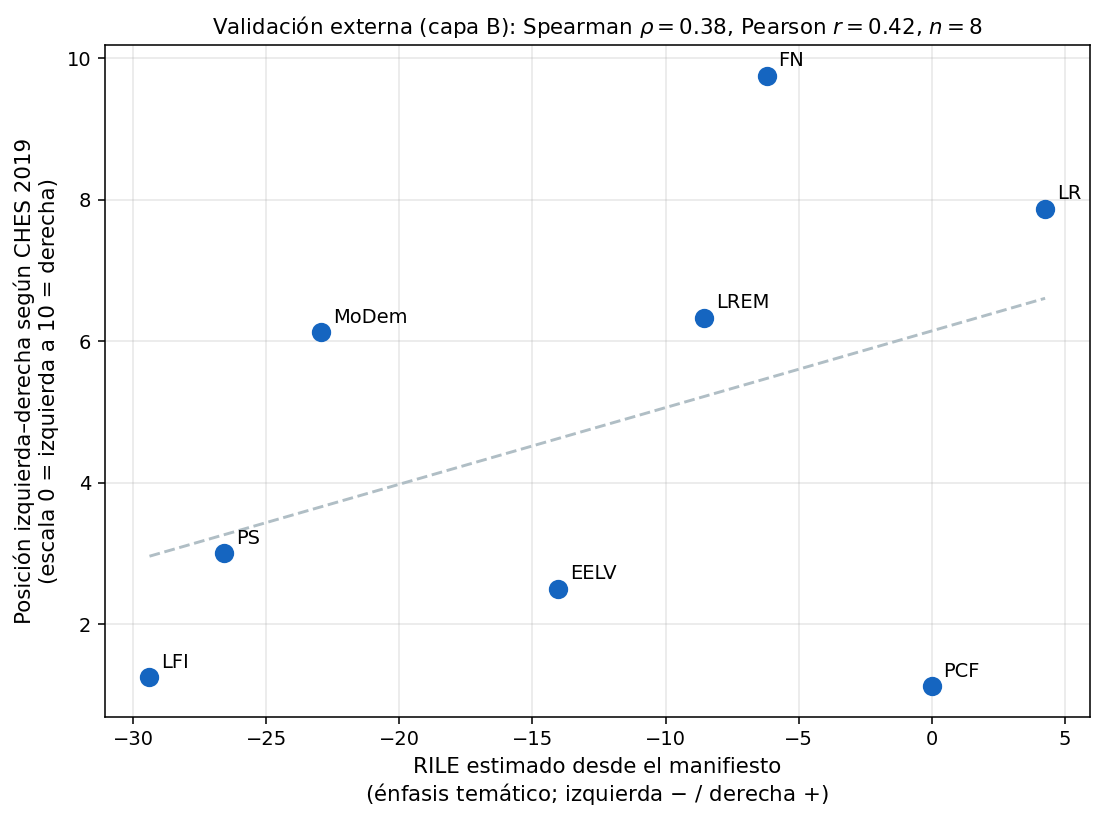
\includegraphics[width=0.82\linewidth]{imagenes/scatter_rile_vs_ches.png}
\caption{RILE estimado por el modelo (eje horizontal) frente a la ubicación
izquierda--derecha del CHES~2019 (\texttt{lrgen}, eje vertical) para los ocho
partidos emparejables (capa B, $\rho \approx 0{,}38$, $n=8$). La línea
discontinua marca la tendencia.}
\label{fig:rile-ches}
\end{figure}

\subsection{Alcance de la validación}
\label{sec:res-val-alcance}

La evidencia anterior debe leerse con varias salvedades que acotan su alcance.
La más importante es que \textbf{la validación solo puede hacerse sobre los
manifiestos}, porque son el único canal con codificación humana MARPOR y el
único con un \emph{benchmark} de expertos comparable. No existe un \emph{ground
truth} equivalente para tuits, intervenciones, leyes o enmiendas, de modo que la
calidad de la clasificación en esas arenas se asume por transferencia desde el
desempeño observado en los manifiestos, no se mide directamente.

En segundo lugar, todas estas correlaciones descansan sobre \textbf{un
número muy pequeño de partidos} (entre 6 y 10, y solo entre 6 y 8 en las capas
que involucran al CHES), por lo que son sensibles a casos individuales y deben
interpretarse como indicios de validez y no como estimaciones precisas; de ahí el
uso de correlación de rangos y el reporte sistemático del $n$. A esa fragilidad contribuyen además las \textbf{muestras
pequeñas} de algunos manifiestos: el PCF aporta apenas 39 cuasi-frases y el PS,
79, por lo que sus posiciones estimadas son solo indicativas. Se suma un
\textbf{desfase temporal} asumido: la referencia de expertos corresponde a 2019
y los manifiestos a las elecciones de 2017, una diferencia de dos años que puede
introducir discrepancias menores sin invalidar la comparación.

Por último, conviene reiterar que el RILE se emplea aquí \textbf{únicamente como
instrumento de validación externa}, no como eje del análisis. Es un índice
posicional unidimensional, frágil y ciego a la dirección del enunciado, por lo
que resulta inadecuado para caracterizar agendas ricas y multidimensionales. El
análisis sustantivo de los partidos, que se desarrolla en las secciones
siguientes, se construye en cambio sobre el \emph{énfasis temático} ---las
distribuciones completas de categorías y dominios MARPOR \cite{marpor_mp_v5}---
y no sobre este eje izquierda--derecha. En síntesis, la validación respalda usar
las predicciones del pipeline como base de los análisis temáticos: el
clasificador reproduce la codificación humana al agregar por partido y, con
suficiente texto, recupera posiciones que se aproximan a las de un panel
independiente de expertos.

\section{Las bases de datos construidas}
\label{sec:res-bases}
% Cobertura y volumen por corpus; tablas resumen.

\section{Agenda declarada: el canal define de qué se habla}
\label{sec:res-declarada}
% Hallazgo transversal: manifiestos = programa (Welfare); tweets/hemiciclo =
% meta-política (Political System). La firma distintiva de cada partido persiste.

\subsection{Manifiestos}
\label{sec:res-manifestos}
% Firmas por partido (EELV->ambiente, PS->bienestar, FN->nación, ...). Caveats de muestra.
% \begin{figure}[H] \centering \includegraphics[width=\linewidth]{...} \caption{...} \end{figure}

\subsection{Twitter}
\label{sec:res-tweets}
% Political System estalla; LFI como megáfono anti-gobierno; NI -> ley y orden.

\subsection{Hemiciclo}
\label{sec:res-hemiciclo}
% La oposición fiscaliza (305 Autoridad Política); LREM defiende gestión (303).

\section{Agenda revelada por el voto}
\label{sec:res-revelada}

\subsection{Dos capas del voto: posicional y temática}
\label{sec:res-dos-capas}
% Leyes invierten la estructura de apoyo respecto de enmiendas (gobierno vs oposición).

\subsection{Cohesión: quién vota en bloque}
\label{sec:res-cohesion}
% LFI la más disciplinada; NI y LT las menos cohesionadas (bolsas mixtas).

\subsection{Clivajes ideológicos en las enmiendas}
\label{sec:res-clivajes}
% Eje cultural (Fabric of Society) vs. libertades (Freedom & Democracy); consenso exterior.

\section{Declarado vs. revelado: ¿votan lo que dicen?}
\label{sec:res-declarado-revelado}
% Tipología por celda (énfasis respaldado / coherencia negativa / oposicional);
% coherencia agregada débil; la estructura interpretable está en los signos por celda.

\chapter{Discusión}
\label{cap:discusion}

% Capítulo optativo (ver manual FCFM, sección 2.4). Interpreta y contrasta los
% resultados con la literatura del marco teórico. Si se prefiere, esta discusión
% puede integrarse dentro de Resultados y eliminarse este capítulo.

\section{Interpretación de los hallazgos}
\label{sec:disc-interpretacion}
% Qué dicen los resultados sobre la coherencia discurso/voto; issue ownership.

\section{Validez del enfoque MARPOR + NLP}
\label{sec:disc-validez}
% El clasificador reproduce identidades partidarias conocidas (validación cualitativa);
% límites de RILE y por qué el énfasis es más robusto.

\section{Limitaciones}
\label{sec:disc-limitaciones}
% Muestras chicas (PCF, PS), duplicaciones (LR/UDI), grupos heterogéneos (NI, LT),
% comparabilidad entre canales, alcance a Francia.

\chapter{Conclusiones}
\label{cap:conclusiones}

% Responde a ¿qué?: evalúa si se cumplieron los objetivos, presenta los principales
% hallazgos, aprendizajes y proyecciones.

\section{Cumplimiento de los objetivos}
\label{sec:concl-objetivos}

\section{Principales hallazgos}
\label{sec:concl-hallazgos}
% El gap declarado-vs-revelado como aporte central; firmas que persisten por canal.

\section{Contribuciones}
\label{sec:concl-contribuciones}
% Bases de datos públicas, documentadas y replicables; pipeline de análisis.

\section{Trabajo futuro}
\label{sec:concl-futuro}
% Extensión a Chile; stance detection; marcos de valores (Schwartz, MFT);
% análisis a nivel de diputado; KG-Gen sobre el corpus completo.


% \input{glosario.tex} % opcional

\bibliographystyle{plain}
\bibliography{bibliografia}

\begin{appendices}
\chapter{Material complementario}
\label{anexo:a}

% Los anexos contienen información complementaria que, por su extensión o naturaleza,
% no se incluye en el cuerpo principal: tablas extensas, detalles de los datos,
% configuraciones de los modelos, figuras adicionales, etc.

\section{Detalle de los corpus y filtros}
\label{anexo:corpus}
% Volúmenes por fuente, filtros mínimos por familia política, consolidación de grupos.

\section{Taxonomía MARPOR: dominios y categorías}
\label{anexo:marpor}
% Tabla con los 7 dominios y las 56 categorías.

\section{Validación del clasificador}
\label{anexo:validacion}
% Accuracy top-1/top-3 y matriz de confusión contra cmp_code humano.

\section{Tópicos de BERTopic por corpus}
\label{anexo:bertopic}

Este anexo complementa la sección~\ref{sec:res-bertopic} del capítulo de
resultados. Recoge, para cada uno de los cinco corpus, los \textbf{24 tópicos
finales} descubiertos por BERTopic \cite{grootendorst2022bertopic} tras la
reducción a un número comparable de tópicos, ordenados de mayor a menor tamaño.
La columna \emph{Tema} es una lectura humana del tópico; las
\emph{palabras representativas} son los términos de mayor peso c-TF-IDF
producidos por el modelo (en francés, lengua del corpus). Los tópicos señalados
como \emph{residuales} o \emph{procedimentales} recogen sobre todo lenguaje de
forma (fórmulas administrativas, mecánica de votos o de sesión) antes que
contenido político, y deben leerse con esa salvedad. Por tratarse de un análisis
exploratorio, estos tópicos no alimentan las métricas a nivel de partido.

{\footnotesize
\begin{longtable}{@{}r r >{\raggedright\arraybackslash}p{0.34\linewidth} >{\raggedright\arraybackslash}p{0.40\linewidth}@{}}
\caption{Tópicos de BERTopic en los manifiestos (3.801 cuasi-frases; 24 tópicos;
1.169 \emph{outliers}).}\label{tab:bt-manifestos}\\
\toprule
\textbf{\#} & \textbf{Docs} & \textbf{Tema} & \textbf{Palabras representativas} \\
\midrule
\endfirsthead
\multicolumn{4}{@{}l}{\footnotesize\itshape (continuación del Cuadro~\ref{tab:bt-manifestos})}\\
\toprule
\textbf{\#} & \textbf{Docs} & \textbf{Tema} & \textbf{Palabras representativas} \\
\midrule
\endhead
\bottomrule
\endlastfoot
0 & 436 & Francia / Europa / proyecto nacional & france, europe, françaises, européens, européenne \\
1 & 304 & Constitución y reforma institucional & parlement, constitution, législative, parlementaire, démocratie \\
2 & 284 & Educación / sistema escolar & enseignement, pédagogiques, système scolaire, supérieur, écoles \\
3 & 226 & Fiscalidad / jubilaciones & évasion fiscale, petites retraites, pensions, impôt revenu \\
4 & 178 & Servicios públicos y territorio & services publics, fonctions publiques, aménagement territoire \\
5 & 164 & Trabajo / derechos del asalariado & droits salariés, contrat travail, employeur, heures supplémentaires \\
6 & 163 & Familia / asignaciones / salud familiar & allocations familiales, quotient familial, maisons santé \\
7 & 125 & Agricultura ecológica / PAC & agriculture écologique, politique agricole, agriculture biologique \\
8 & 94 & Energías renovables / transición & énergies renouvelables, éolien, transition énergétique \\
9 & 79 & Soberanía digital / numérique & numérique, souveraineté numérique, révolution numérique \\
10 & 78 & Economía social y solidaria & économie sociale, sociale solidaire, utilité sociale \\
11 & 76 & Crítica política / república / outre-mer & défi politique, ruine économique, démagogique, république \\
12 & 74 & Igualdad mujeres-hombres & égalité femmes, droits femmes, libertés femmes \\
13 & 53 & Marítimo / outre-mer & océans, économie mer, ports français, maritime \\
14 & 51 & Asilo e inmigración & demandes asile, droit asile, immigration, migrants \\
15 & 41 & Pleno empleo / poder adquisitivo & agir pouvoir, contrat, plein-emploi, laïcité \\
16 & 36 & Lucha contra el terrorismo & contre terrorisme, antiterroriste, terroristes djihadistes \\
17 & 36 & Justicia / prisiones / penas & peines plancher, prison, places prison, recidiviste \\
18 & 32 & Lemas de campaña & gagnerons, sommes prêts, sommes capables \\
19 & 28 & «Aucune fatalité» / lemas & aucune fatalité, ruralite, vie rien \\
20 & 21 & Energía nuclear / disuasión & nucléaire, dissuasion nucléaire, mix énergétique \\
21 & 20 & Reducción del empleo público & supprimerons emplois publics, réduirons nombre \\
22 & 17 & TPE-PME & tpe, plan tpe, tpe pme, simplification \\
23 & 16 & Deporte & sport, fédérations sportives, pratique sportive \\
\end{longtable}
}

{\footnotesize
\begin{longtable}{@{}r r >{\raggedright\arraybackslash}p{0.34\linewidth} >{\raggedright\arraybackslash}p{0.40\linewidth}@{}}
\caption{Tópicos de BERTopic en las enmiendas (2.575 enmiendas; 24 tópicos;
656 \emph{outliers}).}\label{tab:bt-amendements}\\
\toprule
\textbf{\#} & \textbf{Docs} & \textbf{Tema} & \textbf{Palabras representativas} \\
\midrule
\endfirsthead
\multicolumn{4}{@{}l}{\footnotesize\itshape (continuación del Cuadro~\ref{tab:bt-amendements})}\\
\toprule
\textbf{\#} & \textbf{Docs} & \textbf{Tema} & \textbf{Palabras representativas} \\
\midrule
\endhead
\bottomrule
\endlastfoot
0 & 222 & Fiscalidad / impuestos & impôts amendement, général impôts, fiscale, impôt, taxe additionnelle \\
1 & 187 & Vivienda / construcción & logement, logements, construction habitation, logements sociaux, immobilier \\
2 & 153 & Procedimiento penal / prisión & ans emprisonnement, procédure pénale, peines, pénale, emprisonnement \\
3 & 119 & Derecho del trabajo / representación de asalariados & administrateurs salariés, représentant salariés, employeurs, salarié \\
4 & 114 & Reforma de jubilaciones & réformes retraites, système retraites, régime retraite, retraite universel \\
5 & 111 & Alimentación / pesca / rural & denrées alimentaires, rural pêche, pêche maritime, produits agricoles \\
6 & 99 & Educación / autoridad parental & autorité parentale, matière éducation, pédagogiques, établissements enseignement \\
7 & 88 & Salud / médicos / acceso a cuidados & médecins généralistes, santé publique, professionnels santé, assurance maladie \\
8 & 82 & Carta del medio ambiente & charte environnement, environnementale, protection environnement \\
9 & 73 & Financiamiento / presupuesto & financements, budgétaire, financement, budget, euros crédits \\
10 & 64 & Inmigración / extranjeros / asilo & immigration intégration, immigration, migrants, étrangers droit, droit asile \\
11 & 63 & Forma del \emph{amendement} (procedimental) & amendement groupe, amendement propose, mandat député \\
12 & 62 & Lemas políticos / represión & répression institutionnalisé, projet demandons, dévastateur amendement \\
13 & 61 & Pedidos de informe (mecanismos parlamentarios) & rapport évalue, rapport évaluant, demande rapport, rapport information \\
14 & 59 & Fórmula «souligner/justifier» (procedimental) & texte amendement, amendement souligner, solennellement amendement, amendement justifie \\
15 & 59 & Reforma constitucional & inscrire constitution, 24 constitution, suffrages exprimés, élections législatives \\
16 & 58 & Fórmula «suivants/sauf» (procedimental) & texte suivants, suivants sauf, deuxième, sauf accord \\
17 & 48 & Crisis sanitaria / estado de urgencia & crise sanitaire, juillet 2022, urgence sanitaire, mai 2021, état urgence \\
18 & 48 & COVID-19 / vacunación & covid 19, résultat sérologique, schéma vaccinal, virus, couverture vaccinale \\
19 & 41 & Transportes públicos & 1115 transports, transports publics, transport ferroviaire, transport routier \\
20 & 31 & Discriminación / federaciones deportivas & contre discriminations, er constitution, société mentionnée, fédérations sportives \\
21 & 30 & Libertades digitales / neutralidad de la red & libertés numériques, privée numérique, neutralité internet, liberté expression \\
22 & 24 & Reciclaje de plásticos & recyclage bouteilles, bouteilles plastique, bouteilles consommées, plastique usage \\
23 & 23 & Prestaciones sociales / discapacidad & prestations familiales, compensation handicap, bénéficiaires, justice sociale \\
\end{longtable}
}

{\footnotesize
\begin{longtable}{@{}r r >{\raggedright\arraybackslash}p{0.34\linewidth} >{\raggedright\arraybackslash}p{0.40\linewidth}@{}}
\caption{Tópicos de BERTopic en las leyes (23.267 párrafos; 24 tópicos;
8.833 \emph{outliers}). El tópico 0, dominante (${\sim}36\,\%$ del corpus), y los
tópicos 7, 10 y 16 son boilerplate residual.}\label{tab:bt-lois}\\
\toprule
\textbf{\#} & \textbf{Docs} & \textbf{Tema} & \textbf{Palabras representativas} \\
\midrule
\endfirsthead
\multicolumn{4}{@{}l}{\footnotesize\itshape (continuación del Cuadro~\ref{tab:bt-lois})}\\
\toprule
\textbf{\#} & \textbf{Docs} & \textbf{Tema} & \textbf{Palabras representativas} \\
\midrule
\endhead
\bottomrule
\endlastfoot
0 & 8.349 & Boilerplate de informes (residual) & rapport, mentionnés, mentionné, mesures \\
1 & 1.201 & Fiscalidad intercomunal / colectividades territoriales & intercommunale fiscalité, public coopération, collectivités territoriales \\
2 & 815 & Educación / formación profesional & enseignement, formation professionnelle, éducation, apprentis \\
3 & 648 & Política de desarrollo / solidaridad mundial & politique développement, développement solidaire, inégalités mondiales \\
4 & 565 & Déficit / crisis / proyección presupuestaria & déficit, crise, 2020, 2024 \\
5 & 275 & Renovación energética / construcción / vivienda & rénovation énergétique, construction habitation, production énergie \\
6 & 265 & Ley PACTE 2019 & 2019 croissance, transformation entreprises, croissance transformation \\
7 & 265 & Boilerplate fiscal (residual) & mentionnée 2e, réfaction mentionnée, engagements exprimés \\
8 & 245 & Fiscalidad / tasa profesional & taxe professionnelle, fiscalité, etat profit \\
9 & 238 & Elecciones / electoral & élections partielles, élections, électoral \\
10 & 235 & Cifras y montos (residual) & colonne montant, 23 162, suivantes 000 \\
11 & 210 & Promulgación presidencial (fórmula) & président promulgue, visa président \\
12 & 177 & Financiamiento / contribuciones / dependencia & 000 contribution, financement, dépenses solde \\
13 & 171 & Asilo y derecho de los refugiados & demande asile, droit asile, protection réfugiés \\
14 & 164 & Especialidades farmacéuticas / salud & spécialité pharmaceutique, prescription, chargés santé \\
15 & 122 & Autopistas y rutas & autoroutes, autoroutes routes, voies transférées \\
16 & 74 & Cifras presupuestarias (residual) & montant arrondi, conjoncturel mesures \\
17 & 70 & Base del impuesto / imposición & assiette impôt, imposition cas, droits organisme \\
18 & 66 & Outre-mer / Pacífico & futuna, polynésie wallis, futuna, art 765 \\
19 & 59 & Pensión de reversión / jubilación & retraite cas, pension réversion, retraite obligatoire \\
20 & 57 & «France Services» / red de servicios & france services, services public, maisons services \\
21 & 57 & Asociaciones / federaciones deportivas & sport statuts, association sportive, fédération sportive \\
22 & 54 & Capacidad eléctrica (kW) & 000 kw, 750 kw, 500 kw \\
23 & 52 & Controles aduaneros / dinero en efectivo & argent liquide, contrôles argent, européen \\
\end{longtable}
}

{\footnotesize
\begin{longtable}{@{}r r >{\raggedright\arraybackslash}p{0.34\linewidth} >{\raggedright\arraybackslash}p{0.40\linewidth}@{}}
\caption{Tópicos de BERTopic en los tuits (222.644 tuits; 24 tópicos;
105.894 \emph{outliers}).}\label{tab:bt-tweets}\\
\toprule
\textbf{\#} & \textbf{Docs} & \textbf{Tema} & \textbf{Palabras representativas} \\
\midrule
\endfirsthead
\multicolumn{4}{@{}l}{\footnotesize\itshape (continuación del Cuadro~\ref{tab:bt-tweets})}\\
\toprule
\textbf{\#} & \textbf{Docs} & \textbf{Tema} & \textbf{Palabras representativas} \\
\midrule
\endhead
\bottomrule
\endlastfoot
0 & 15.662 & Guerra de Ucrania / Rusia & ukrainien, ukraine, peuple ukrainien, russie, guerre \\
1 & 15.444 & Reuniones públicas / agenda local & réunion, assemblée nationale, rencontre, citoyens \\
2 & 11.501 & Macron / presidencia & emmanuel macron, macron, françois bayrou, président \\
3 & 11.104 & Juegos Olímpicos / deporte & jeux olympiques, olympique, champions, athlètes \\
4 & 9.462 & Francia / France Insoumise / elecciones europeas & france insoumise, françaises, élections européennes \\
5 & 7.320 & Reforma de jubilaciones & réforme retraites, pensions, retraités, sécurité sociale \\
6 & 6.190 & Fin de vida / cuidados paliativos / eutanasia & soins palliatifs, aide mourir, palliatifs, euthanasie \\
7 & 5.855 & Mundo agrícola / Salon de l'Agriculture & monde agricole, soutien agriculteurs, salon agriculture \\
8 & 5.853 & Policía / inseguridad / acoso & contre harcèlement, policiers, police, violence \\
9 & 5.472 & Política energética / transición / nuclear & politique énergétique, transition énergétique, énergies renouvelables \\
10 & 4.945 & Condolencias / homenajes / fallecimientos & sincères condoléances, hommage victimes, immense tristesse \\
11 & 4.292 & Crisis de la vivienda & crise logement, logements sociaux, immobilier \\
12 & 4.227 & Redes sociales / ciberseguridad / 2024-2030 & 2024 2030, cybersécurité, interdiction réseaux sociaux \\
13 & 3.053 & Derechos de las mujeres / 8M & droits femmes, féministes, égalité femmes, women \\
14 & 1.849 & Vacunación COVID-19 & vaccinationcovid, campagne vaccination, stratégie vaccinale \\
15 & 1.024 & Saludos de fin de año & belle année, bonne année, joyeux noël \\
16 & 969 & Anuncios de invitaciones a medios & invité serai, 8h30 invité, serai invité \\
17 & 847 & Bomberos & hommage pompiers, pompiers volontaires, sapeurs pompiers \\
18 & 574 & Venezuela / Maduro & peuple vénézuélien, venezuela, débarrassé dictature \\
19 & 370 & China / diplomacia & ambassadeur chine, china, régime chinois \\
20 & 324 & Iglesia católica / papa & pape américain, nouveau pape, pontificat \\
21 & 175 & Autismo (sensibilización) & sensibilisation autisme, semaine autisme, personnes autistes \\
22 & 134 & Afganistán / talibanes & situation afghanistan, kaboul afghanistan, afghanes talibans \\
23 & 104 & Cannabis / despenalización & cannabis dépénalisation, légaliser cannabis, légalisation cannabis \\
\end{longtable}
}

{\footnotesize
\begin{longtable}{@{}r r >{\raggedright\arraybackslash}p{0.34\linewidth} >{\raggedright\arraybackslash}p{0.40\linewidth}@{}}
\caption{Tópicos de BERTopic en las intervenciones del hemiciclo
(338.192 intervenciones; 24 tópicos; 165.439 \emph{outliers}). Los tópicos 0, 1,
9, 11 y 17 son procedimentales o residuales.}\label{tab:bt-interventions}\\
\toprule
\textbf{\#} & \textbf{Docs} & \textbf{Tema} & \textbf{Palabras representativas} \\
\midrule
\endfirsthead
\multicolumn{4}{@{}l}{\footnotesize\itshape (continuación del Cuadro~\ref{tab:bt-interventions})}\\
\toprule
\textbf{\#} & \textbf{Docs} & \textbf{Tema} & \textbf{Palabras representativas} \\
\midrule
\endhead
\bottomrule
\endlastfoot
0 & 40.135 & Discurso político genérico (procedimental-residual) & parlementaire, parlementaires, parce, politique \\
1 & 31.080 & Comisión / dictamen (procedimental-residual) & républicains demande, commission suis, avis commission \\
2 & 24.483 & Unión Europea / Europa & union européenne, europe, européens, gouvernement \\
3 & 22.754 & Reforma / presupuesto / gobierno & réforme, gouvernement, budget, politique \\
4 & 15.125 & Sistema de salud / sanitario & système santé, urgence sanitaire, professionnels santé \\
5 & 8.128 & Educación / escuela & directeurs école, scolaires, écoles \\
6 & 3.493 & Desempleo / seguro de desempleo & chômage, chômeurs, demandeurs emploi, assurance chômage \\
7 & 3.482 & Transporte ferroviario & ferroviaires, ferroviaire, transports \\
8 & 3.455 & Derechos de las mujeres / igualdad & droits femmes, égalité femmes, sages femmes, sexistes \\
9 & 3.046 & Resultados de votos (procedimental-residual) & nombre votants, suffrages exprimés \\
10 & 2.713 & Agua / agencias del agua & agences eau, gestion eau, accès eau, eau assainissement \\
11 & 2.685 & «Renvoyée à la prochaine séance» (procedimental) & prochaine, renvoyée prochaine, prochaine demande \\
12 & 2.547 & Medios / audiovisual público & médias, journalistes, audiovisuel public \\
13 & 2.047 & Deporte / asociaciones deportivas & associations sportives, ministère sports, clubs sportifs \\
14 & 1.538 & Notre-Dame / patrimonio & restauration cathédrale, cathédrale dame, église \\
15 & 1.122 & Política exterior / Siria / Argelia & syrie, algérie, affaires étrangères, armées \\
16 & 1.094 & Bioética / embriones & embryon humain, souches embryonnaires, lois bioéthique \\
17 & 1.040 & Llamadas al reglamento (procedimental) & rappels règlement, rappel règlement, règles \\
18 & 940 & Maltrato animal / protección animal & maltraitance animale, animal compagnie, protection animale \\
19 & 595 & Lengua / lenguas regionales & langue république, langues régionales, langue régionale \\
20 & 543 & Constitucional / artículos & articles constitutionnelle, poursuivi articles \\
21 & 294 & COVID / mascarillas & acheter masques, masque obligatoire, porter masque \\
22 & 253 & Cifras / «milliards d'euros» (residual) & milliards euros, million euros \\
23 & 161 & Mención personal (residual) & caroline fiat, fiat caroline \\
\end{longtable}
}

Adicionalmente, cada corrida genera una visualización de prevalencia temática por
grupo parlamentario (\texttt{viz\_topics\_per\_political\_group}) para los corpus
de tuits e intervenciones. Estas visualizaciones son interactivas y no se
versionan en el repositorio, por lo que se regeneran ejecutando el pipeline.
% TODO (opcional): si se decide incluir una versión estática, regenerar el
% heatmap de prevalencia de tópicos por grupo (tuits e intervenciones) desde
% bertopic_analysis/<fuente>/results/ y anexarlo aquí.

\subsection{Cruce ilustrativo BERTopic\,$\times$\,MARPOR}
\label{anexo:bertopic-marpor}

A modo de ilustración, la figura~\ref{fig:bertopic-marpor} cruza un tópico de
BERTopic sustantivo del corpus de enmiendas ---el tópico \#2 del
Cuadro~\ref{tab:bt-amendements}, \emph{procedimiento penal / prisión}, dominado
por las expresiones \emph{procédure pénale}, \emph{peines} y
\emph{emprisonnement}--- con la distribución de dominios MARPOR que el
clasificador asigna a esos mismos documentos. Se eligió este tópico por reunir
los criterios fijados de antemano: no es un \emph{outlier}, tiene tamaño
suficiente, no es residual ni meramente procedimental, sus palabras clave son
interpretables y su distribución se concentra de forma apreciable en uno o dos
dominios.

El enlace entre ambas salidas se hace por el \emph{texto} del documento: como las
predicciones de ManifestoBERTa conservan únicamente los primeros 300 caracteres
de cada entrada, ese prefijo opera como clave de unión. Se trata de un enlace
aproximado y no de un identificador documental estable; por eso debe leerse con
cautela. De los \textbf{153} documentos del tópico, \textbf{134} ($87{,}6\,\%$)
pudieron cruzarse con una predicción; los \textbf{19} restantes no encontraron
prefijo coincidente y quedaron fuera. A escala del corpus completo la cobertura
del cruce es del orden del $84\,\%$, y solo tres prefijos resultaron ambiguos
(asociados a más de un dominio) y se descartaron; ninguno de ellos pertenece al
tópico ilustrado, de modo que la distribución mostrada no depende de los casos
excluidos.

La figura \emph{no} valida un modelo con el otro ---son representaciones de
naturaleza distinta y este trabajo no usa una para evaluar la otra---; muestra
únicamente cómo un agrupamiento empírico no supervisado se reparte sobre la
taxonomía supervisada usada en el análisis principal. En este caso predomina, de
forma coherente, el dominio \emph{Fabric of Society} ($73{,}9\,\%$), con una
fracción menor en \emph{Freedom \& Democracy} ($11{,}9\,\%$). La concentración es
interpretable sin sorpresa: en la codificación MARPOR el dominio \emph{Fabric of
Society} agrupa las categorías de orden social y, en particular, la de ley y
orden (605), de modo que las enmiendas sobre penas, prisión y procedimiento penal
se ubican allí; el residuo en \emph{Freedom \& Democracy} recoge el componente de
derechos y garantías que también atraviesa la materia penal. Esta lectura es
ilustrativa y no debe tomarse como evidencia fuerte de alineación entre métodos.

\begin{figure}[htbp]
  \centering
  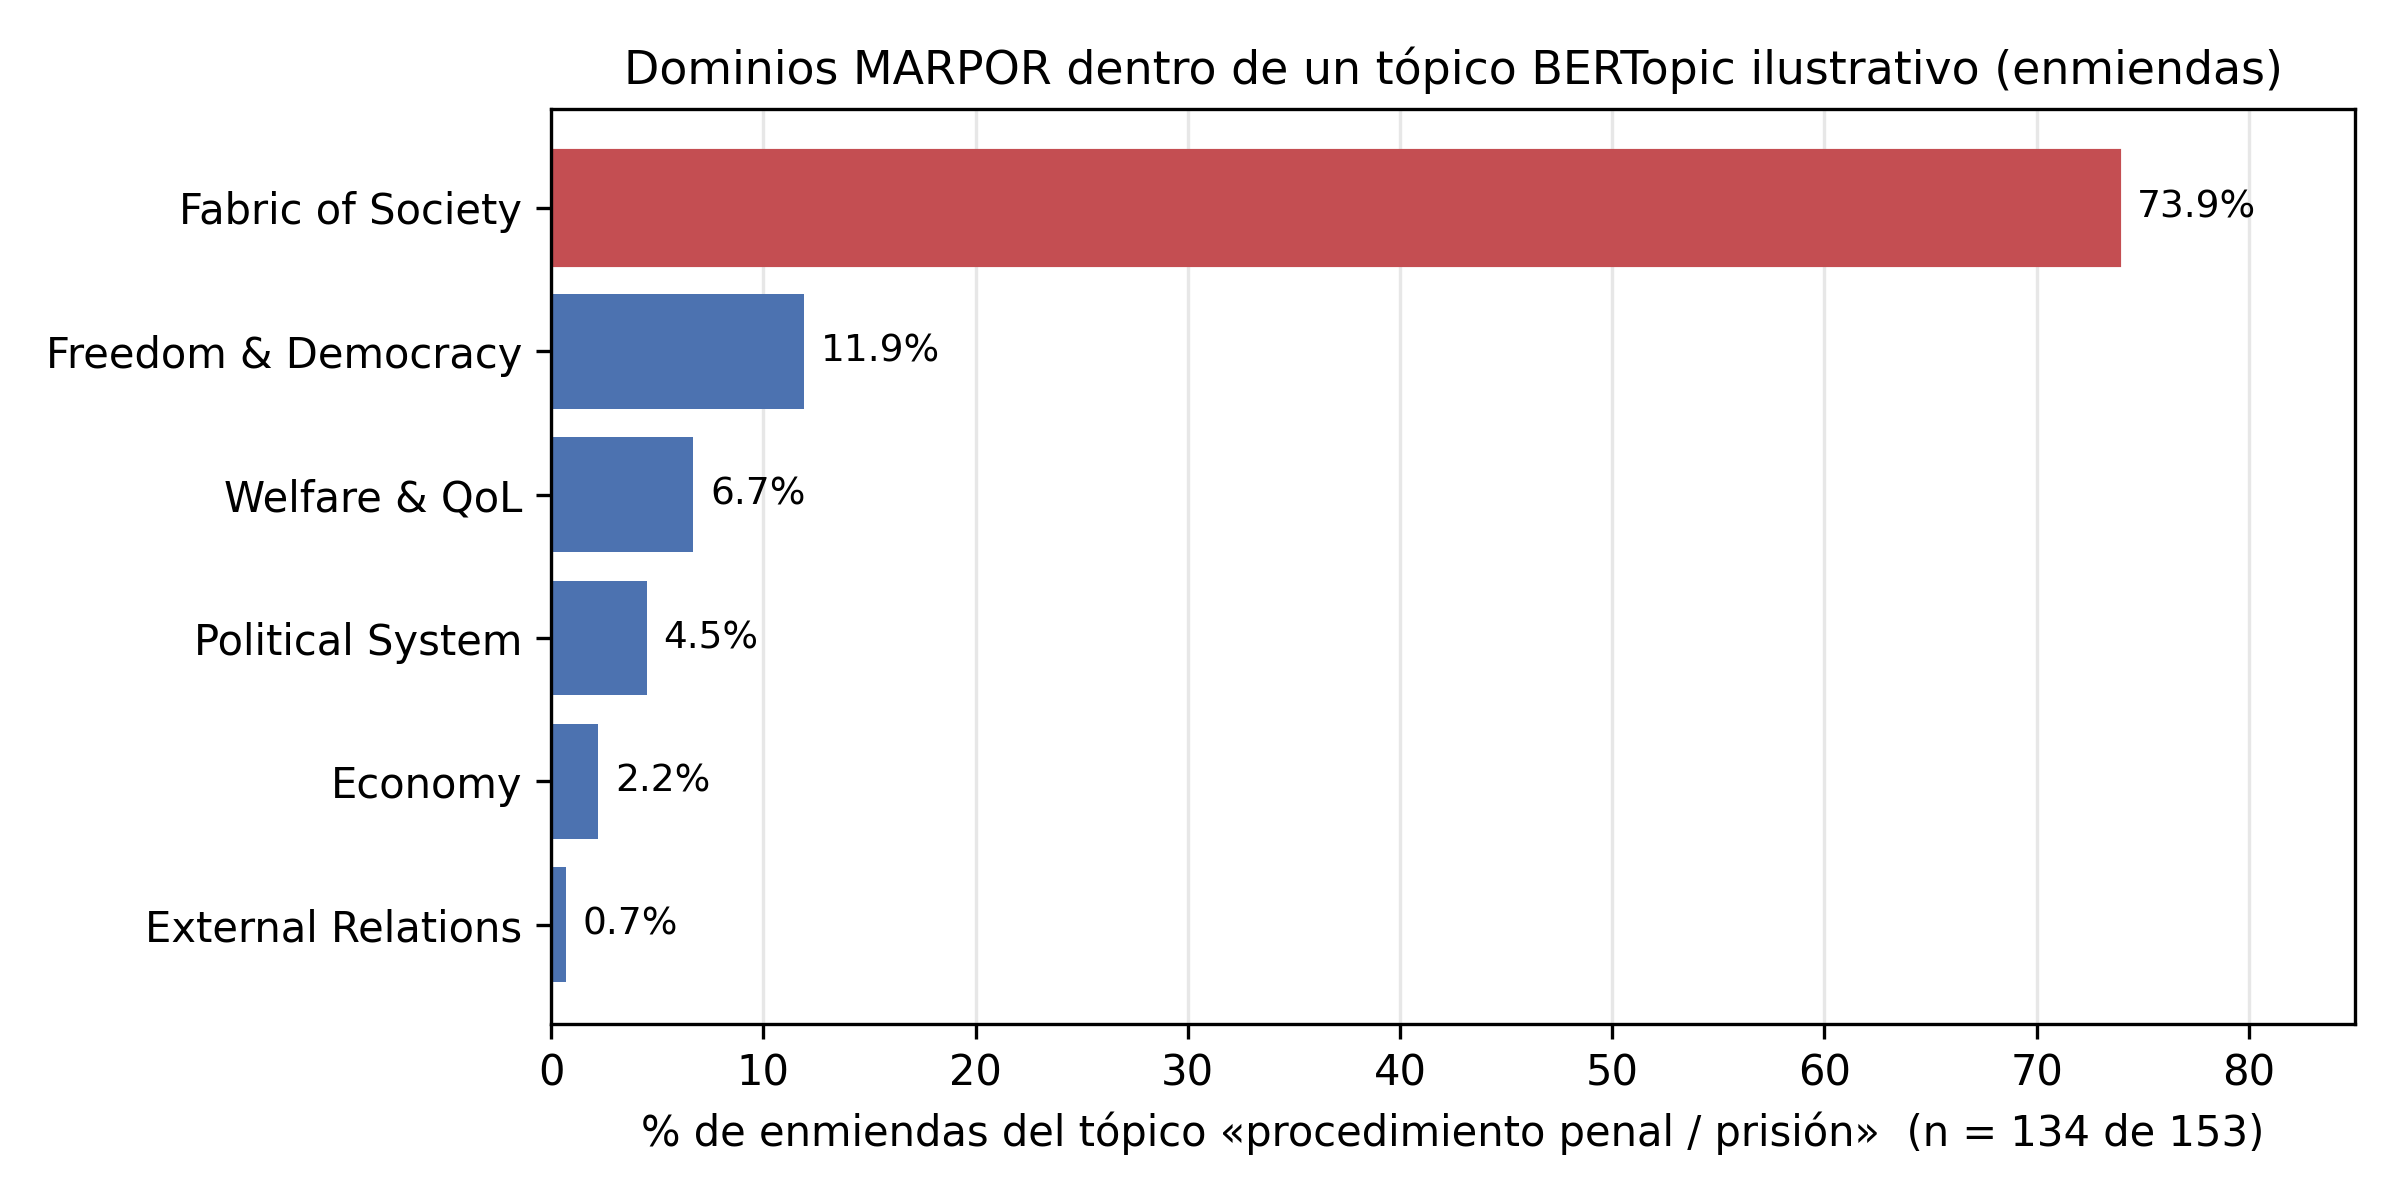
\includegraphics[width=0.85\textwidth]{imagenes/bertopic_marpor_topic_example.png}
  \caption[Cruce ilustrativo BERTopic\,$\times$\,MARPOR]{Distribución de dominios
  MARPOR dentro de un tópico BERTopic ilustrativo: el tópico de enmiendas
  \emph{procedimiento penal / prisión} (134 de 153 documentos enlazados por el
  texto). La figura es ilustrativa y \emph{no} valida un modelo con el otro;
  muestra cómo un agrupamiento empírico no supervisado se distribuye sobre la
  taxonomía supervisada usada en el análisis principal. El enlace se hace por un
  prefijo del texto, por lo que la cobertura es parcial (véase el detalle en el
  cuerpo del anexo).}
  \label{fig:bertopic-marpor}
\end{figure}

\end{appendices}
\end{document}
